% \PassOptionsToPackage{table}{xcolor}
\documentclass[11pt]{beamer}
\usepackage[utf8]{inputenc}
\usepackage[english]{babel}
\usepackage{amsmath}
\usepackage{amsfonts}
\usepackage{amssymb}
\usepackage{graphicx}
\usepackage{tikz}
\usepackage{algorithm}
\usepackage{algorithmic}
\usepackage{silence,lmodern}
\usepackage{csquotes}
\usepackage[backend=bibtex, bibencoding=ascii, style=authoryear, doi=false, isbn=false,url=false, uniquename=init, giveninits=true]{biblatex}
\usepackage{multimedia}
\usepackage{dirtytalk}
\usepackage{pgfplotstable,booktabs,longtable}
\usepackage{grffile}
\usepackage{marvosym} % color image
\WarningFilter{biblatex}{Patching footnotes failed}


% \mode<presentation>
% {
    \usetheme[hideothersubsections]{PaloAlto}
    % \usecolortheme{beaver}
% }
\usetikzlibrary{calc,trees,positioning,arrows,chains,shapes.geometric,
decorations.pathreplacing,decorations.pathmorphing,
shapes,matrix,shapes.symbols,plotmarks,decorations.markings,
shadows,shapes.geometric,arrows}

\setbeamercolor{logo}{bg=white}  %controls the color of the logo area
\setbeamerfont{footnote}{size=\tiny}

% \addbibresource{library.bib}

\makeatletter
\setlength{\beamer@headheight}{.9cm}
\makeatother

\author{S M Al Mahi}
\title[ECEN-5283 Computer Vision]{Project 1: \\Edge Detection}
\setbeamercovered{transparent} 
\setbeamertemplate{navigation symbols}{}


\logo{
\includegraphics[width=1cm]{Oklahoma_State_University_logo.png}}
\institute{Oklahoma State University} 
\date{\today} 
\subject{}
\begin{document}

\setbeamertemplate{sidebar left}{}
\begin{frame}
\titlepage
\end{frame}

\newpage
\setbeamertemplate{sidebar left}[sidebar theme]
\section{Project Objective}
\begin{frame}
\frametitle{Project Objective}
	\begin{block}{Objectives}
	\begin{enumerate}
		\item Implement LoG, Canny and Matched Filter edge detection
		\item Apply them on 4 retinal images for blood vessel detection
		\item Designing kernels for filtering
	\end{enumerate}
	\end{block}
% \end{frame}
% \begin{frame}
	\begin{block}{Tools, Input \& Output}
	\begin{enumerate}
		\item \textbf{Python}, PyCharm IDE, Matplotlib, Numpy
		\item \textbf{Latex Beamer}, Sublime Text
		\item \textbf{Input} Four retina image
	\end{enumerate}
	\end{block}
\end{frame}

\section{Technical Background}
\begin{frame}
\frametitle{Laplacian of Gaussian \textbf{LoG}}
	\begin{enumerate}
		\item Laplacian is the 2D second order derivative  $\operatorname{LoG}(x,y) = \frac{1}{\pi\sigma^4}\left(\frac{x^2+y^2}{2\sigma^2} - 1\right)e^{-\frac{x^2+y^2}{2\sigma^2}}$
		\item LoG is the Laplacian applied to Gaussian ${\rm LoG}(x,y;\sigma)
=
\Delta_{(x,y)}G(x,y;\sigma)
=
\frac{\partial^2 G(x,y;\sigma)}{\partial x^2} + \frac{\partial^2 G(x,y;\sigma)}{\partial y^2}
=
\frac{1}{\pi\sigma^4} \left(\frac{x^2+y^2}{2\sigma^2}-1\right){\rm e}^{-\frac{x^2+y^2}{2\sigma^2}} .$
		\item Instead of calculating Gaussian then Laplacian the kernel is calculated into on single kernel $(K_{\nabla^2}**(G_\sigma **I)) = (K_{\nabla^2**G_\sigma})**I = (\nabla^2G)**I$ 
		\item Thresholding on Zero Crossing is applied to extract only the actual edges 
	\end{enumerate}
\end{frame}

\begin{frame}
\frametitle{Canny}
	\begin{enumerate}
		\item Estimate Gradient to find edges
		\item $f_x=\frac{\delta f}{\delta x}=(K_{\nabla_x^2}**(G_x **I)) = (K_{\nabla_x^2**G_x})**I = (\nabla^2 G_x)**I$ 
		\item $
\Delta_{(x)}G(x;\sigma)
=
\frac{\partial^2 G}{\partial x^2} + \frac{\partial^2 G}{\partial y^2}
=
\frac{-x}{\pi\sigma^4} \left(\frac{x^2+y^2}{2\sigma^2}-1\right){\rm e}^{-\frac{x^2+y^2}{2\sigma^2}} $
		\item $f_y=\frac{\delta f}{\delta y}=(K_{\nabla_y^2}**(G_y **I)) = (K_{\nabla_y^2**G_x})**I = (\nabla^2 G_y)**I$ 
		\item $
\Delta_{(y)}G(y;\sigma)
=
\frac{\partial^2 G}{\partial y^2} + \frac{\partial^2 G}{\partial y^2}
=
\frac{-y}{\pi\sigma^4} \left(\frac{x^2+y^2}{2\sigma^2}-1\right){\rm e}^{-\frac{x^2+y^2}{2\sigma^2}} $
		\item Magnitude of the gradient can tell us whether it is an edge or not $||\nabla f(x,y) ||_2 = \sqrt{f_x(x,y)^2 + f_y(x,y)^2}$
		\item Orientation of the gradient tell us the orientation of the edge $\tan(\theta(x,y)) = \frac{f_y(x,y)}{f_x(x,y)}
\;\;\;
\implies
\;\;\;
\theta(x,y) = \arctan\left( \frac{f_y(x,y)}{f_x(x,y)} \right)$
	\end{enumerate}
\end{frame}


\begin{frame}
\frametitle{Matched filter}
\begin{itemize}
	\item Assumption is that cross section of an edge is Gaussian
	\item $G(x,y) = \frac{1}{2 \pi \sigma ^{2}} e^{- \frac{y^{2}}{2 \sigma ^{2}}} \quad\quad m_0 \in [-x_0, x_0]$
	\item We define a group of filters ${G(x, y)_{\theta1} \dots G(x, y)_{\theta N}}$
	\item Apply these kernel to image and fuse them
	\item We can then threshold the image to get binary image
\end{itemize}
\end{frame}

\section{Results}

\subsection{LoG}
\begin{frame}
\frametitle{Retinal Image Cock wise 1 to 4}
\begin{columns}[T] % align columns
\begin{column}{\textwidth}
\centering
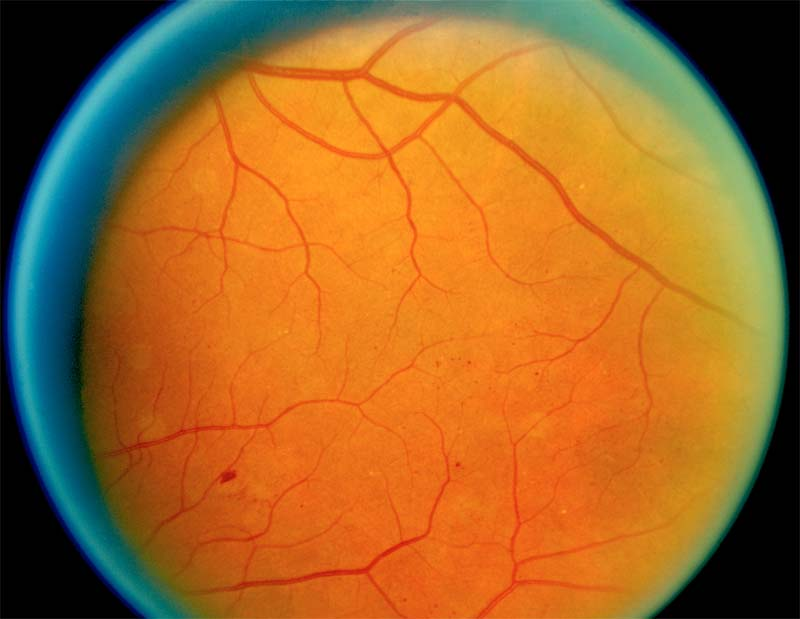
\includegraphics[width=.45\textwidth, height=.45\textheight]{retina1.jpg}\vspace{1pt}
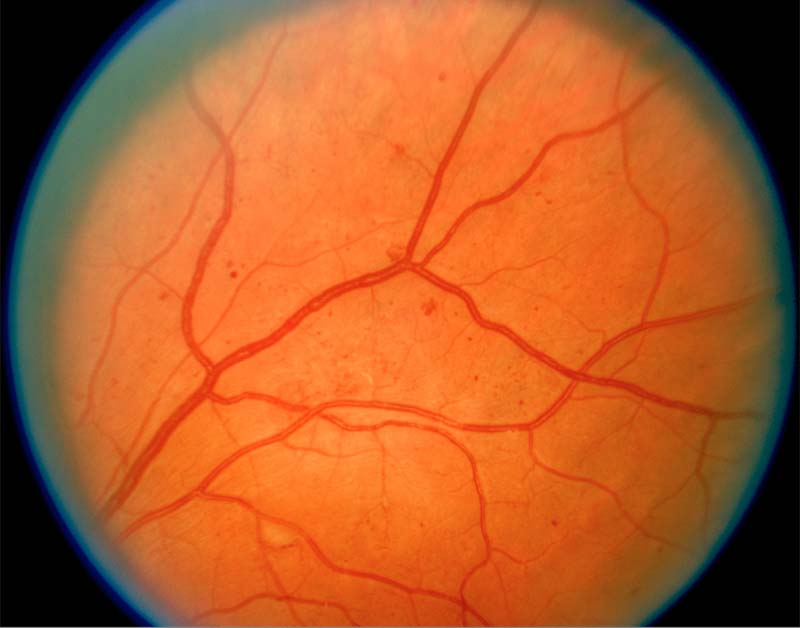
\includegraphics[width=.45\textwidth, height=.45\textheight]{retina2.jpg}\vfill
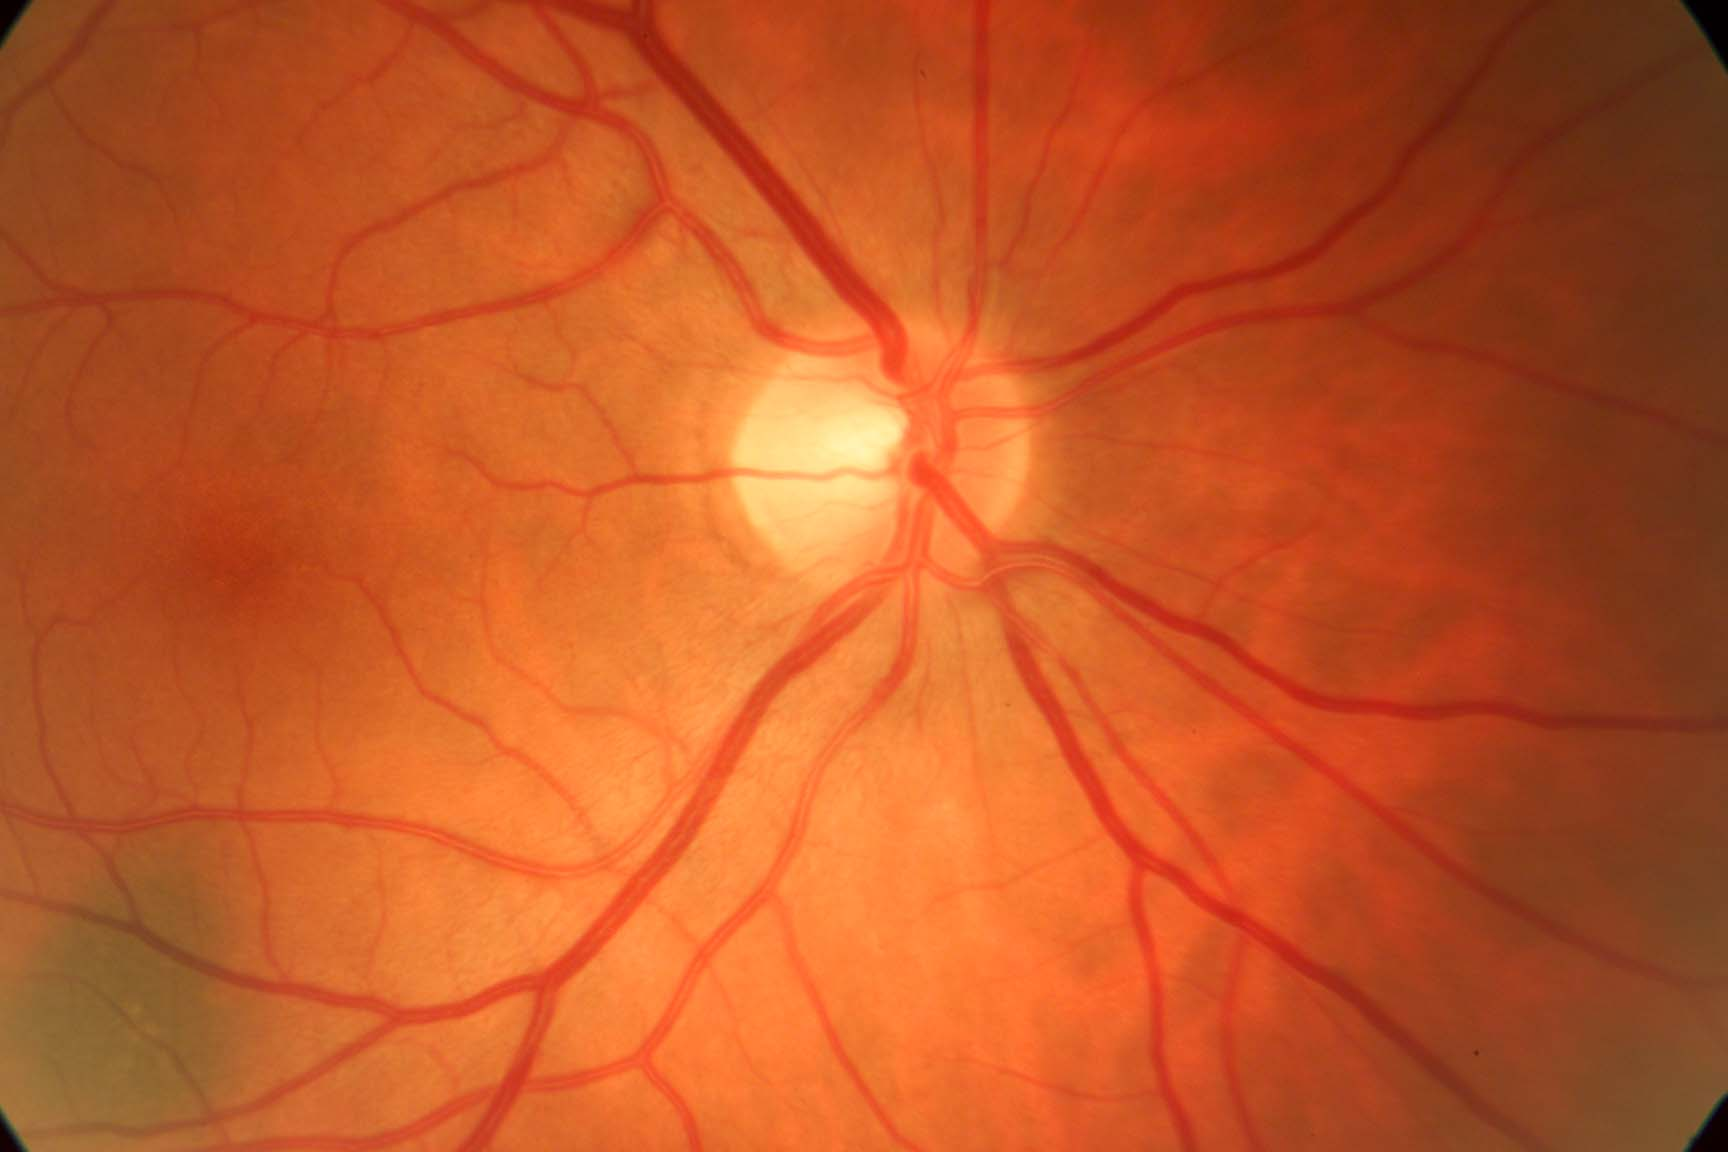
\includegraphics[width=.45\textwidth, height=.45\textheight]{retina3.jpg}\vspace{1pt}
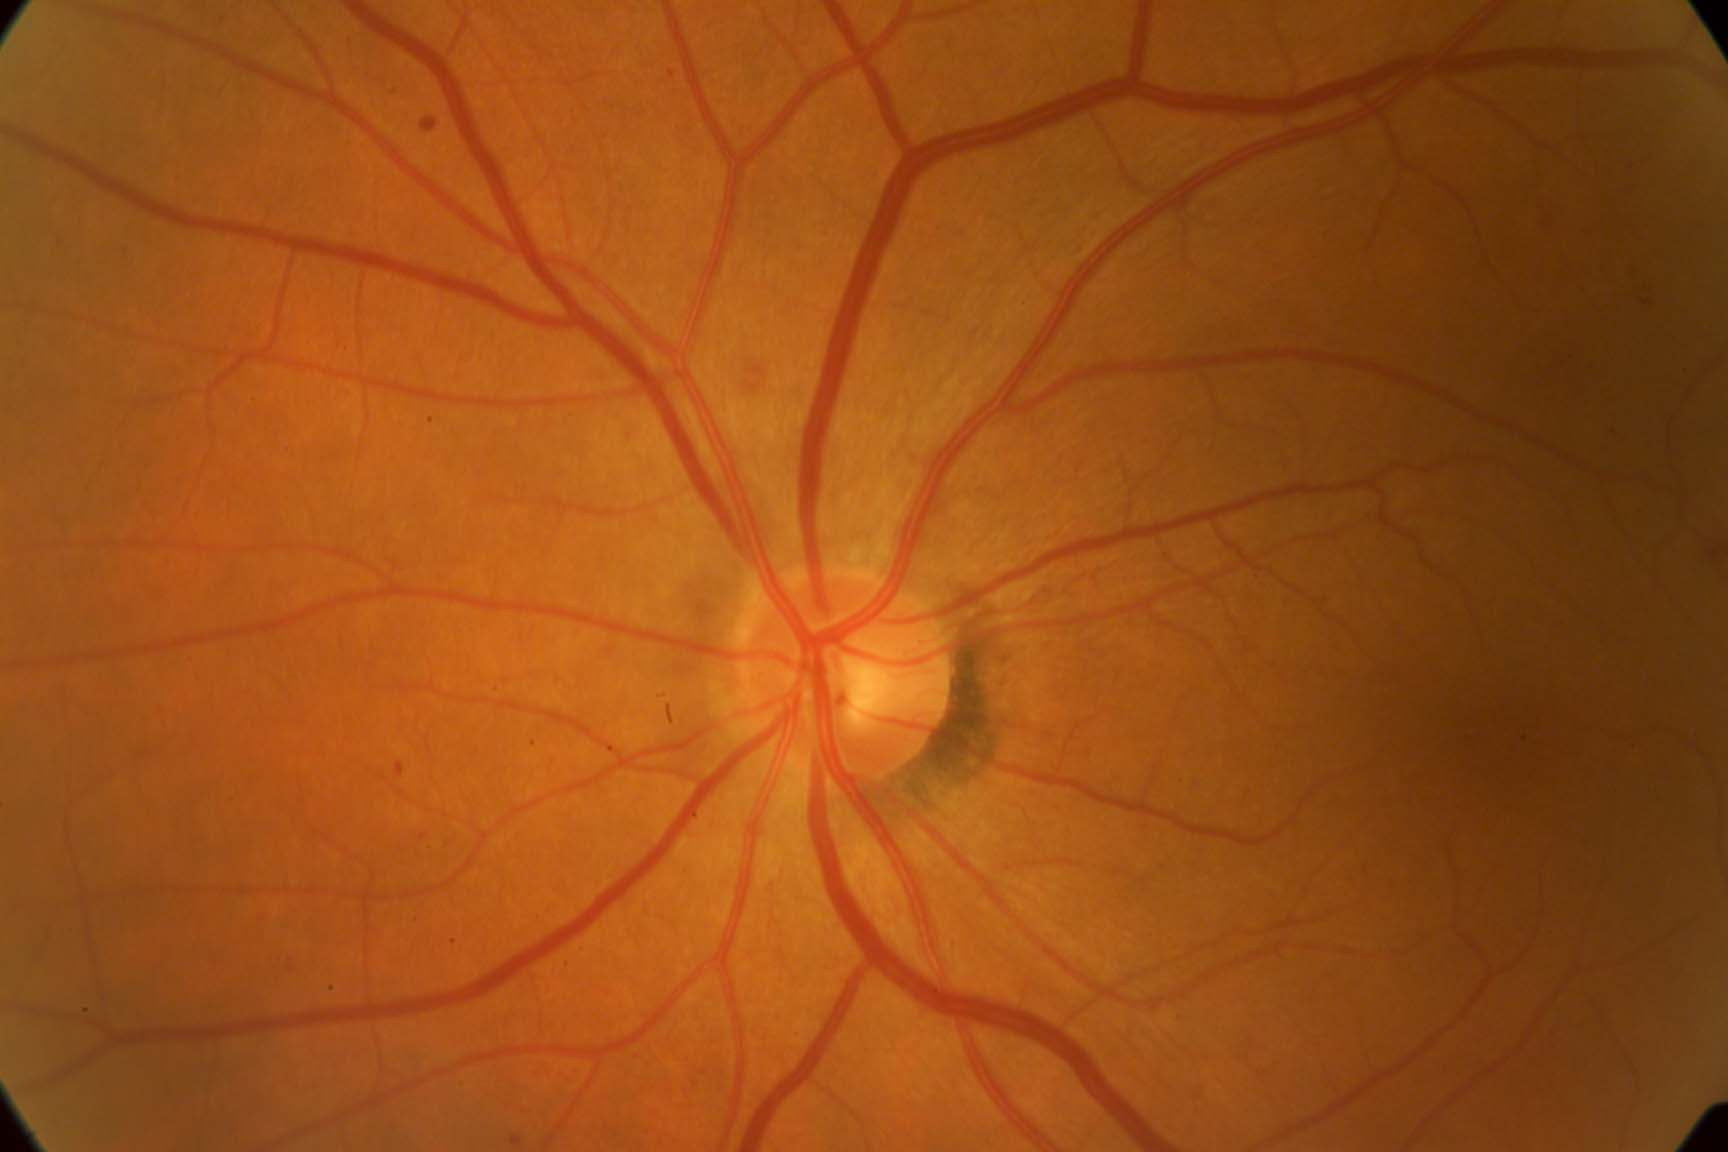
\includegraphics[width=.45\textwidth, height=.45\textheight]{retina4.jpg}\vfill
\end{column}
\end{columns}\vfill
\end{frame}

\begin{frame}
\frametitle{For LoG}
\[
K_2^* =
\begin{bmatrix}
 0 & 0 &   1 & 0 & 0\\
 0 & 1 &   2 & 1 & 0\\
 1 & 2 & -16 & 2 & 1\\
 0 & 1 &   2 & 1 & 0\\
 0 & 0 &   1 & 0 & 0
\end{bmatrix} 
\]\vfill
\[
K_3^* =
\begin{bmatrix}
 0 & 0 &  0 &   1 & 0 & 0 & 0\\
 0 & 0 &  1 &   2 & 1 & 0 & 0\\
 0 & 1 &  1 &  -3 & 1 & 1 & 0\\
 1 & 2 & -3 & -12 &-3 & 2 & 1\\
 0 & 1 &  1 &  -3 & 1 & 1 & 0\\
 0 & 0 &  1 &   2 & 1 & 0 & 0\\
 0 & 0 &  0 &   1 & 0 & 0 & 0
\end{bmatrix} 
\]\vfill
$K_3^*$ has been used for retina3.jpg and retina4.jpg  for LoG while $K_1^*$ for others.
\end{frame}

\begin{frame}
\frametitle{For Canny}
\[
f_x =
\begin{bmatrix}
 0 & 0 & 0 & 0 & 0\\
 0 & 1 & 2 & 1 & 0\\
 0 & 0 & 0 & 0 & 0\\
 0 &-1 &-2 &-1 & 0\\
 0 & 0 & 0 & 0 & 0
\end{bmatrix} 
\]\vfill
\[f_y = f_x^T\]
\begin{itemize}
\item[\color{green}\MVRightarrow] \begin{center} Horizontal orientation \end{center}
\item[\color{blue}\rotatebox{45}{\MVRightarrow}] \begin{center} Positive Slope orientation\end{center}
\item[\color{cyan}\rotatebox{135}{\MVRightarrow}] \begin{center}Negative Slope orientation\end{center}
\item[\color{red}\rotatebox{90}{\MVRightarrow}] \begin{center}Vertical orientation\end{center}
\end{itemize}
\end{frame}

\begin{frame}
\frametitle{For Match}
\begin{itemize}
	\item $m_0 = -0.099$
\end{itemize}
\end{frame}

\begin{frame}
\frametitle{Result and Contrast with Different Parameter}
\begin{columns}[T] % align columns
\begin{column}{\textwidth}
\centering
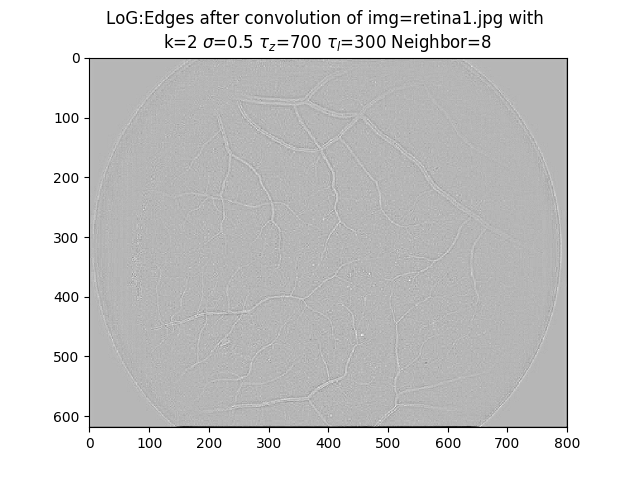
\includegraphics[width=.45\textwidth, height=.45\textheight]{log_fig/retina1.jpg_fig2_0.png}\vspace{1pt}
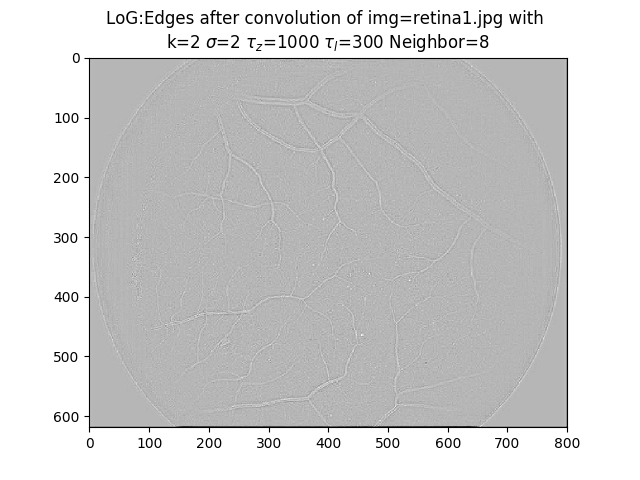
\includegraphics[width=.45\textwidth, height=.45\textheight]{log_fig/retina1.jpg_fig2_4.png}\vfill
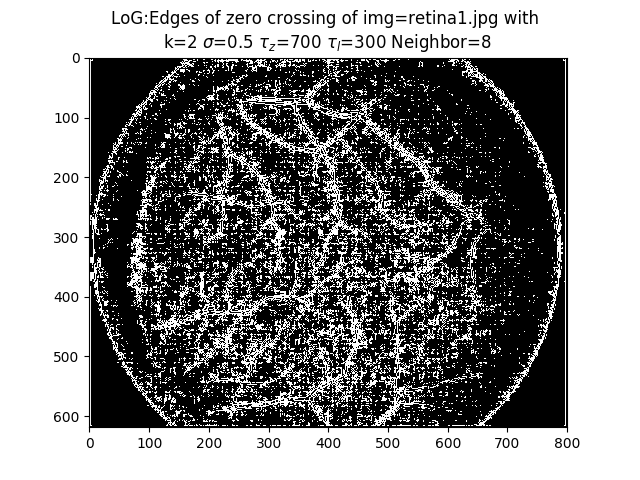
\includegraphics[width=.45\textwidth, height=.45\textheight]{log_fig/retina1.jpg_fig3_0.png}\vspace{1pt}
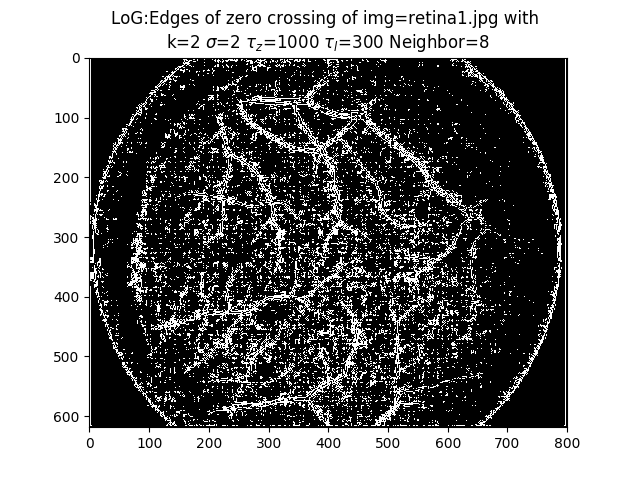
\includegraphics[width=.45\textwidth, height=.45\textheight]{log_fig/retina1.jpg_fig3_4.png}\vfill
\end{column}
\end{columns}\vfill
\end{frame}

\begin{frame}
\frametitle{Result and Contrast with Different Parameter}
\begin{columns}[T] % align columns
\begin{column}{\textwidth}
\centering
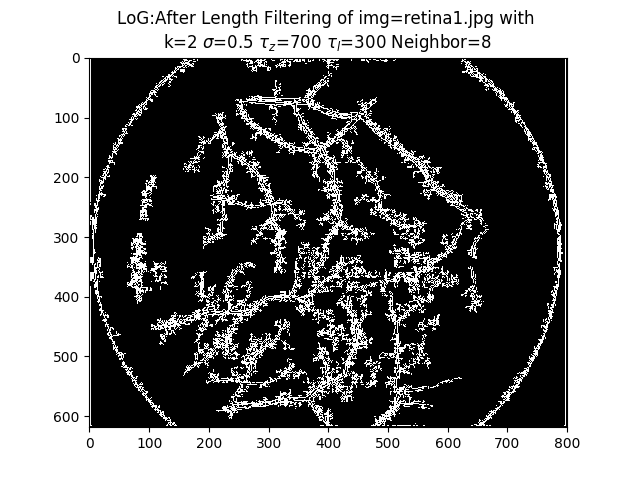
\includegraphics[width=.45\textwidth, height=.45\textheight]{log_fig/retina1.jpg_fig4_0.png}\vspace{1pt}
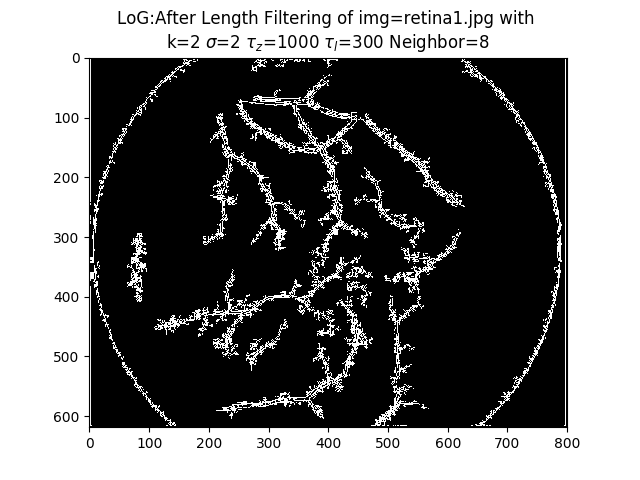
\includegraphics[width=.45\textwidth, height=.45\textheight]{log_fig/retina1.jpg_fig4_4.png}\vfill
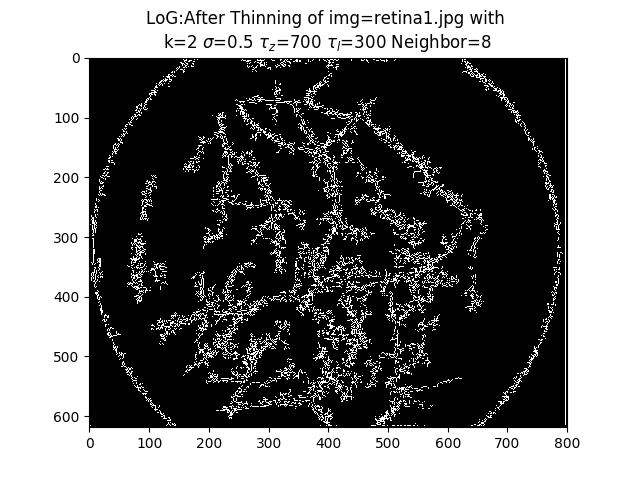
\includegraphics[width=.45\textwidth, height=.45\textheight]{log_fig/retina1.jpg_fig5_0.png}\vspace{1pt}
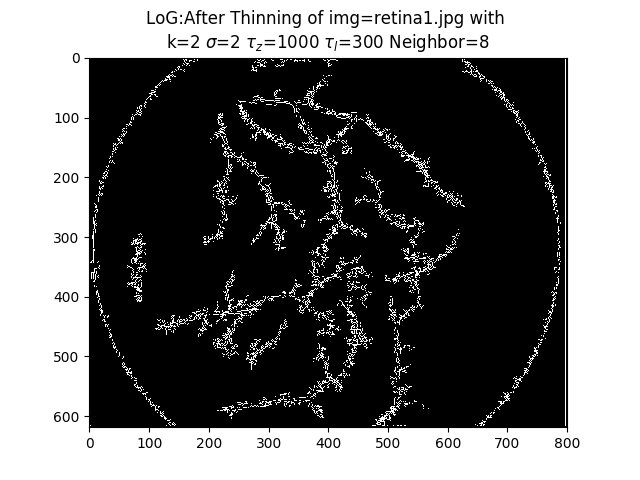
\includegraphics[width=.45\textwidth, height=.45\textheight]{log_fig/retina1.jpg_fig5_4.png}\vfill
\end{column}
\end{columns}\vfill
\end{frame}

\begin{frame}
\frametitle{Result and Contrast with Different Parameter}
\begin{columns}[T] % align columns
\begin{column}{\textwidth}
\centering
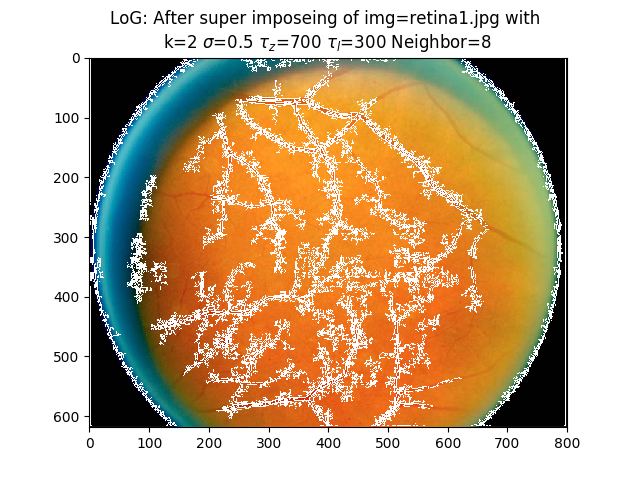
\includegraphics[width=.45\textwidth, height=.45\textheight]{log_fig/retina1.jpg_fig6_0.png}\vspace{1pt}
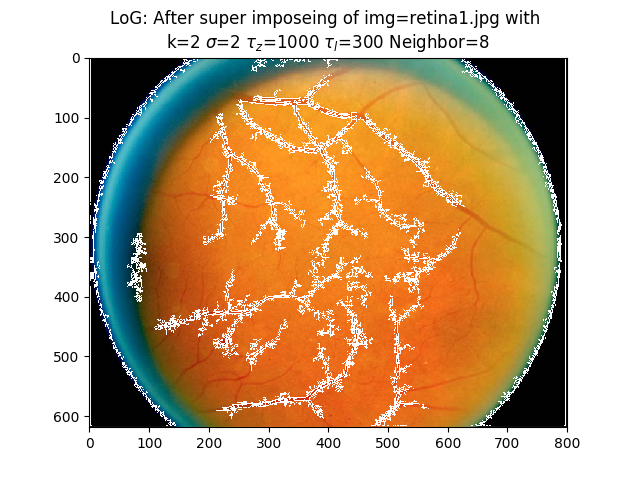
\includegraphics[width=.45\textwidth, height=.45\textheight]{log_fig/retina1.jpg_fig6_4.png}\vfill
% 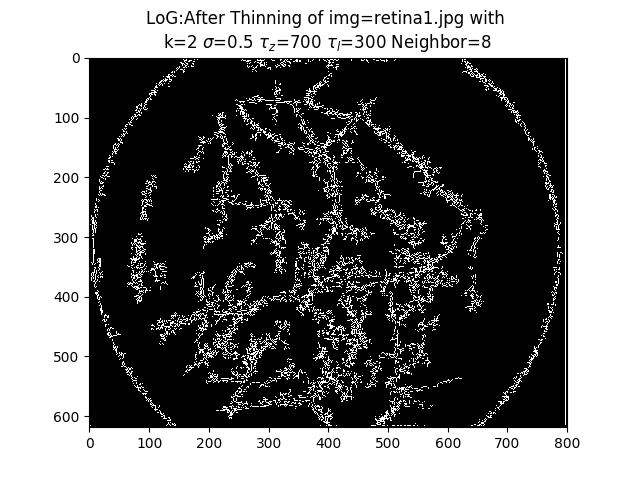
\includegraphics[width=.45\textwidth, height=.45\textheight]{log_fig/retina1.jpg_fig5_0.png}\vspace{1pt}
% 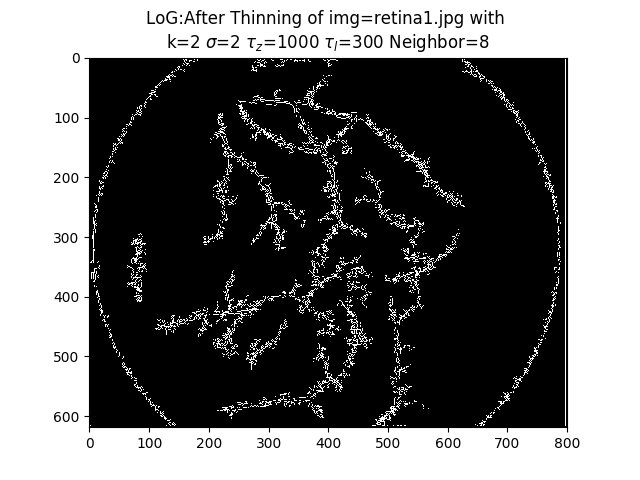
\includegraphics[width=.45\textwidth, height=.45\textheight]{log_fig/retina1.jpg_fig5_4.png}\vfill
\end{column}
\end{columns}\vfill
\end{frame}

\begin{frame}
\frametitle{Result and Contrast with Different Parameter}
\begin{columns}[T] % align columns
\begin{column}{\textwidth}
\centering
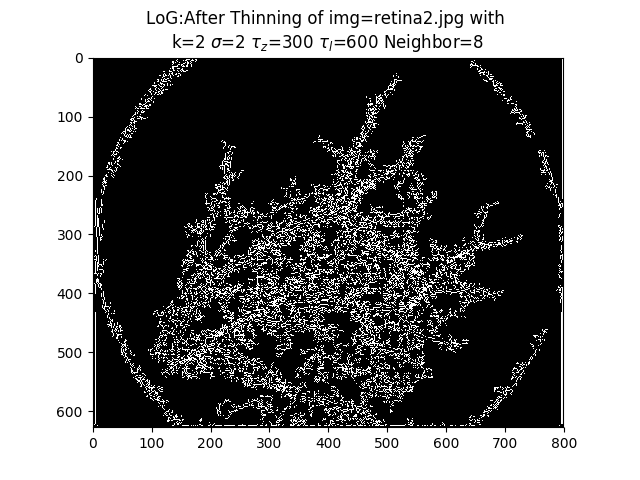
\includegraphics[width=.45\textwidth, height=.45\textheight]{log_fig/retina2.jpg_fig5_5.png}\vspace{1pt}
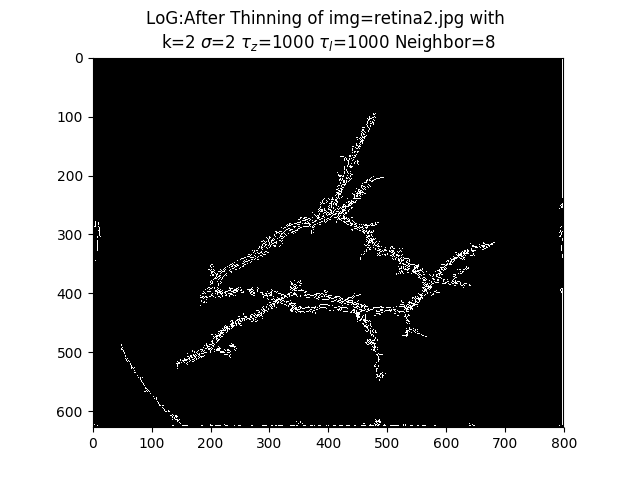
\includegraphics[width=.45\textwidth, height=.45\textheight]{log_fig/retina2.jpg_fig5_6.png}\vfill
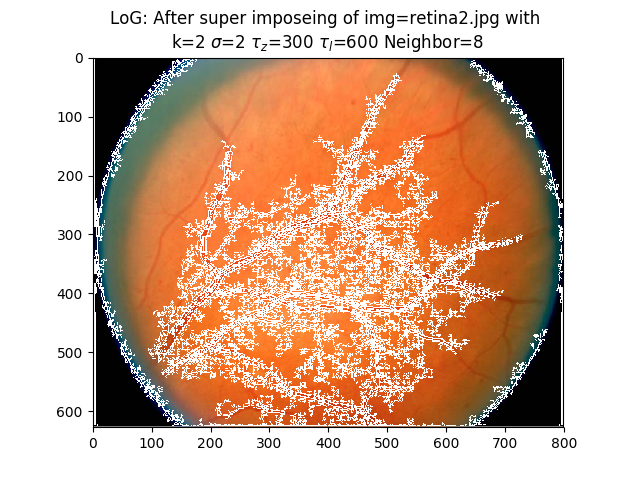
\includegraphics[width=.45\textwidth, height=.45\textheight]{log_fig/retina2.jpg_fig6_5.png}\vspace{1pt}
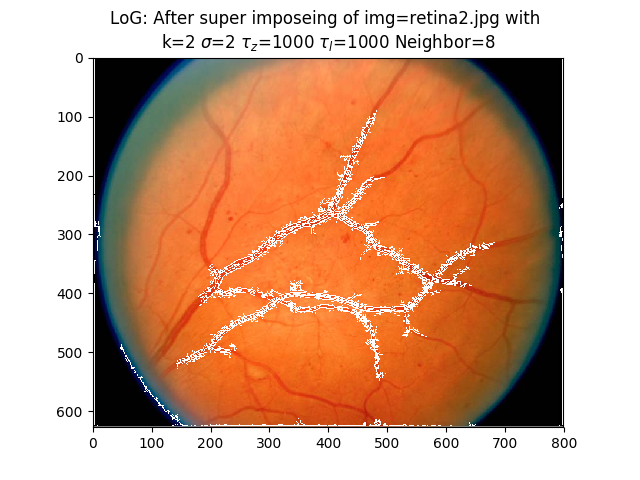
\includegraphics[width=.45\textwidth, height=.45\textheight]{log_fig/retina2.jpg_fig6_6.png}\vfill
\end{column}
\end{columns}\vfill
\end{frame}

\begin{frame}
\frametitle{Result and Contrast with Different Parameter}
\begin{columns}[T] % align columns
\begin{column}{\textwidth}
\centering
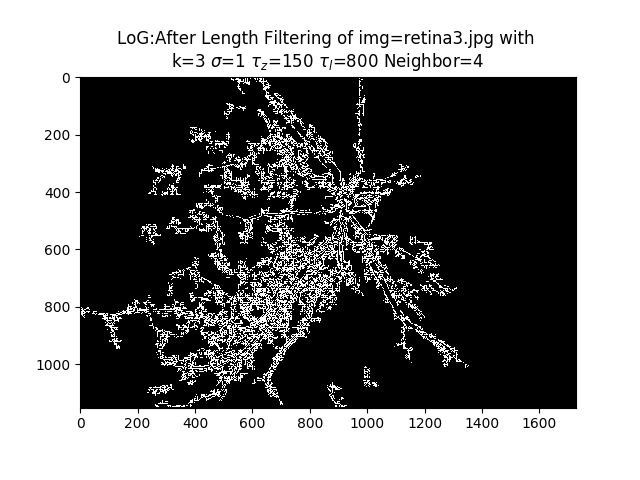
\includegraphics[width=.45\textwidth, height=.45\textheight]{log_fig/retina3.jpg_fig4_3.png}\vspace{1pt}
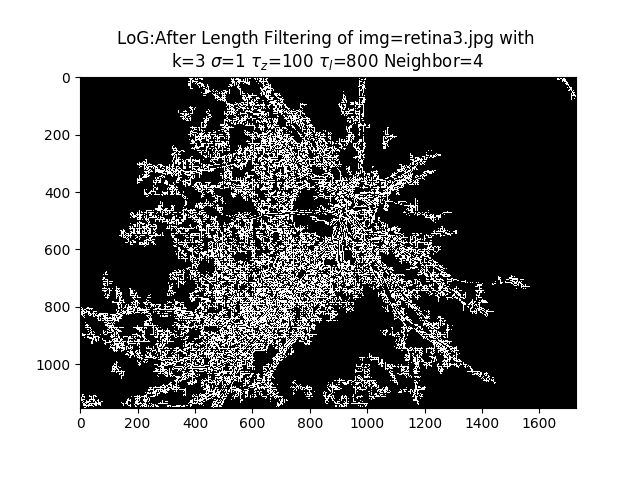
\includegraphics[width=.45\textwidth, height=.45\textheight]{log_fig/retina3.jpg_fig4_7.png}\vfill
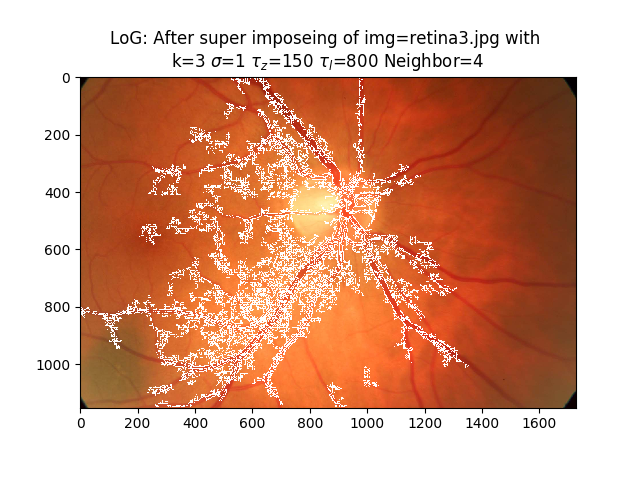
\includegraphics[width=.45\textwidth, height=.45\textheight]{log_fig/retina3.jpg_fig6_3.png}\vspace{1pt}
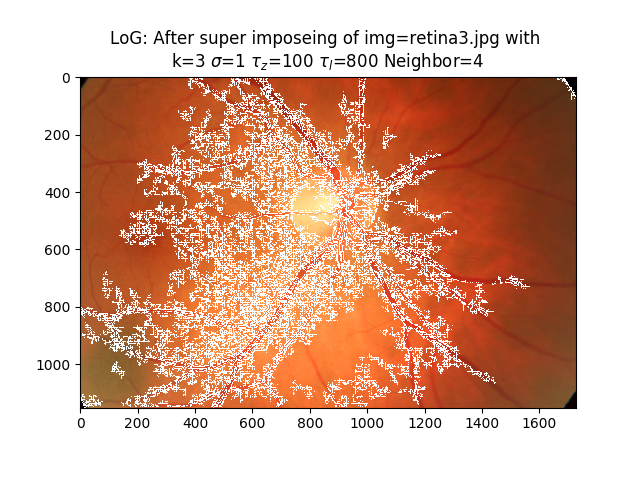
\includegraphics[width=.45\textwidth, height=.45\textheight]{log_fig/retina3.jpg_fig6_7.png}\vfill
\end{column}
\end{columns}\vfill
\end{frame}

\begin{frame}
\frametitle{Result and Contrast with Different Parameter}
\begin{columns}[T] % align columns
\begin{column}{\textwidth}
\centering
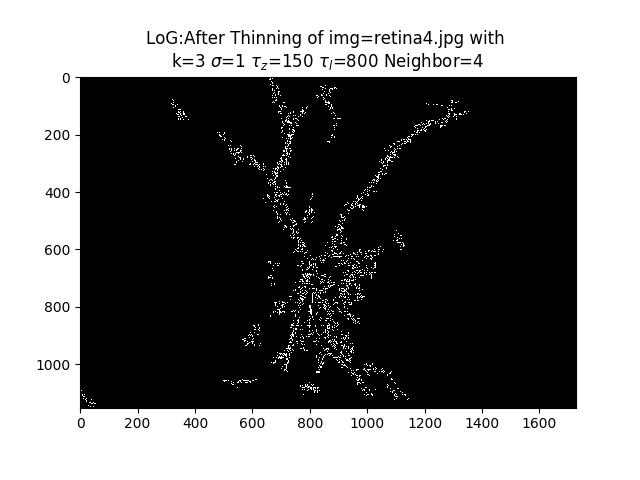
\includegraphics[width=.45\textwidth, height=.45\textheight]{log_fig/retina4.jpg_fig5_4.png}\vspace{1pt}
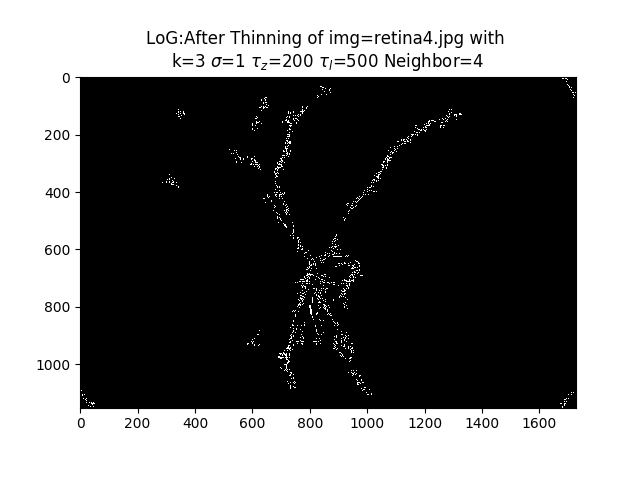
\includegraphics[width=.45\textwidth, height=.45\textheight]{log_fig/retina4.jpg_fig5_8.png}\vfill
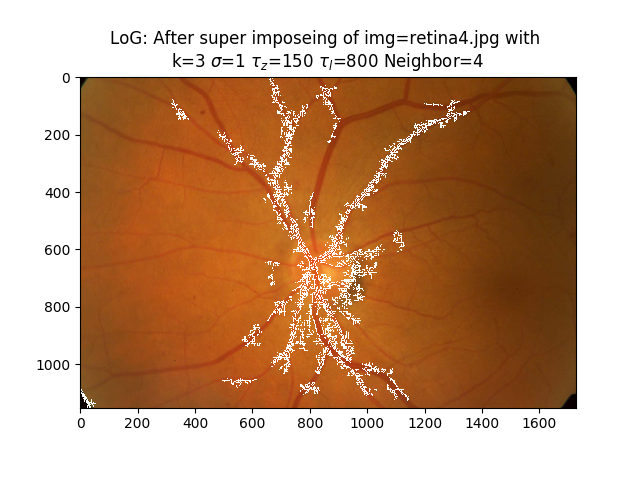
\includegraphics[width=.45\textwidth, height=.45\textheight]{log_fig/retina4.jpg_fig6_4.png}\vspace{1pt}
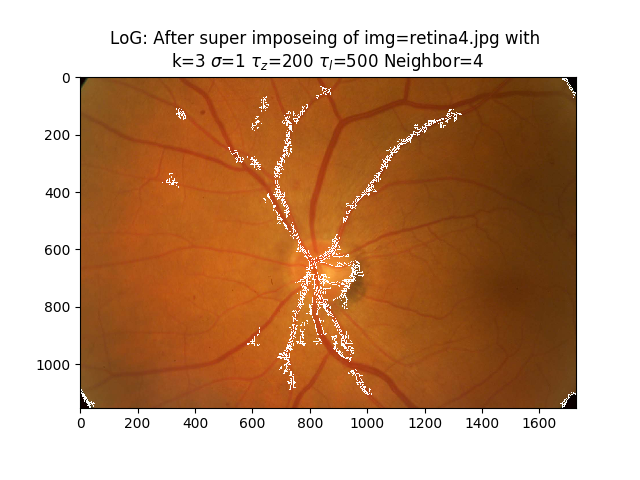
\includegraphics[width=.45\textwidth, height=.45\textheight]{log_fig/retina4.jpg_fig6_8.png}\vfill
\end{column}
\end{columns}\vfill
\end{frame}

\subsection{Canny}
\begin{frame}
\frametitle{\textbf{Canny:} Result and Contrast with Diff Param}
\begin{columns}[T] % align columns
\begin{column}{\textwidth}
\centering
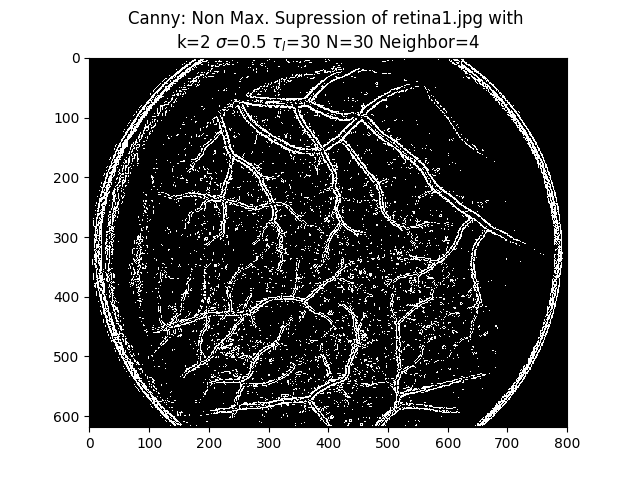
\includegraphics[width=.45\textwidth, height=.45\textheight]{canny_fig/retina1.jpg_fig2_0.png}\vspace{1pt}
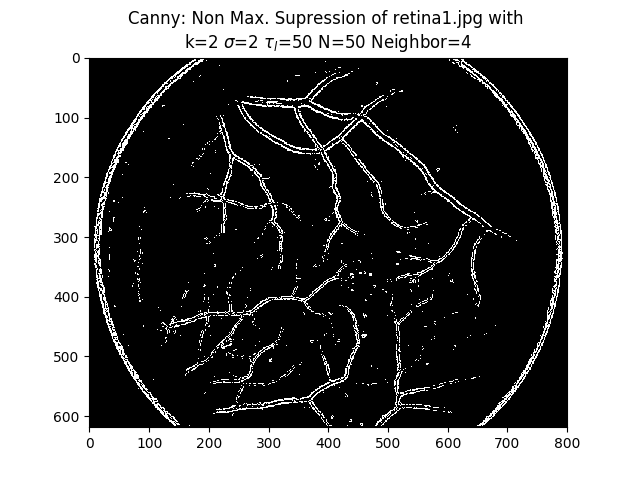
\includegraphics[width=.45\textwidth, height=.45\textheight]{canny_fig/retina1.jpg_fig2_4.png}\vfill
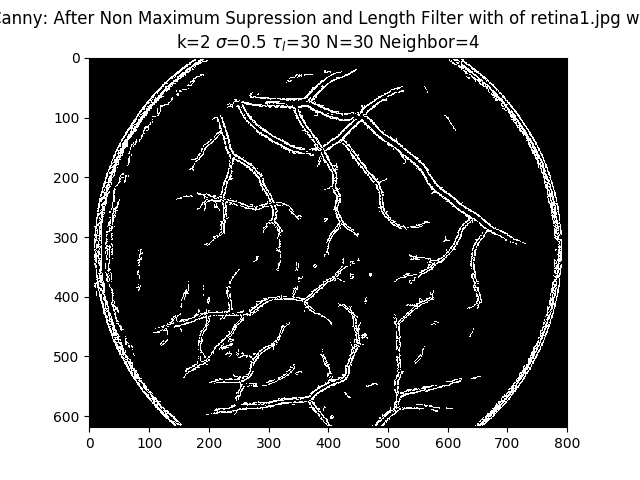
\includegraphics[width=.45\textwidth, height=.45\textheight]{canny_fig/retina1.jpg_fig3_0.png}\vspace{1pt}
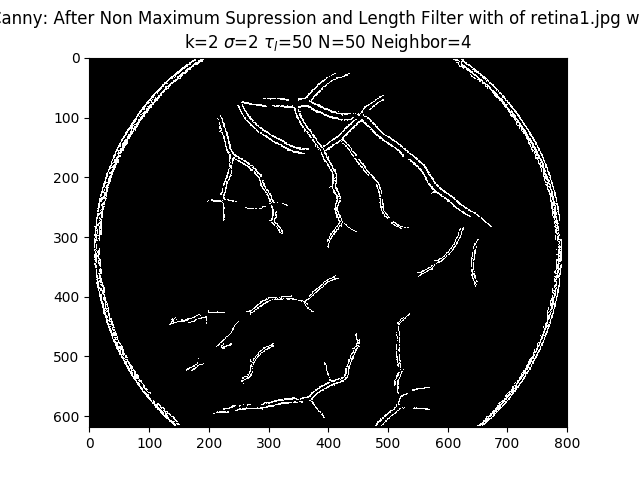
\includegraphics[width=.45\textwidth, height=.45\textheight]{canny_fig/retina1.jpg_fig3_4.png}\vfill
\end{column}
\end{columns}\vfill
\end{frame}

\begin{frame}
\frametitle{\textbf{Canny:} Result and Contrast }
\begin{columns}[T] % align columns
\begin{column}{\textwidth}
\centering
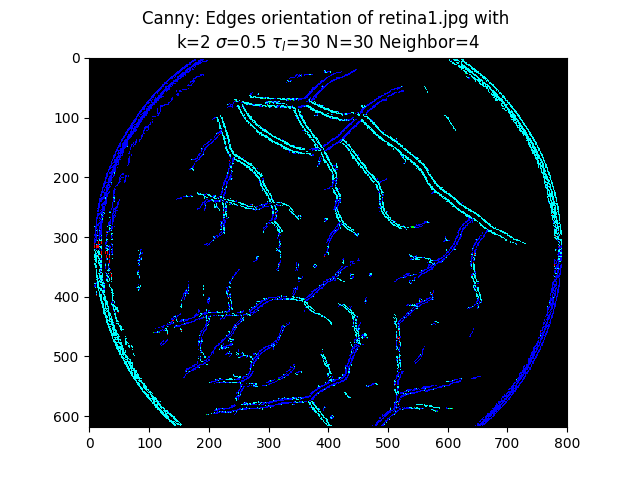
\includegraphics[width=.45\textwidth, height=.45\textheight]{canny_fig/retina1.jpg_fig4_0.png}\vspace{1pt}
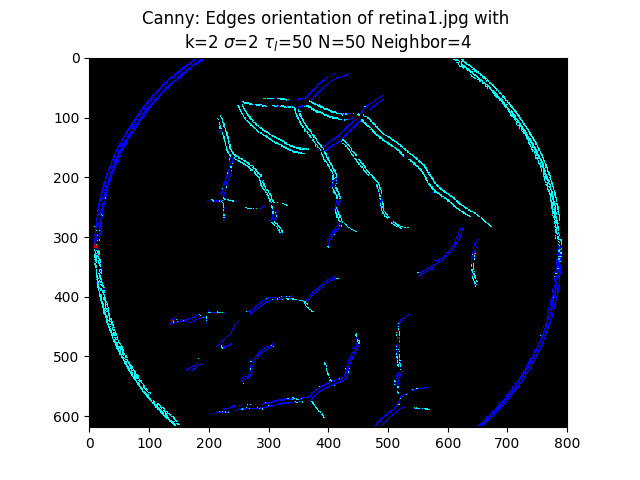
\includegraphics[width=.45\textwidth, height=.45\textheight]{canny_fig/retina1.jpg_fig4_4.png}\vfill
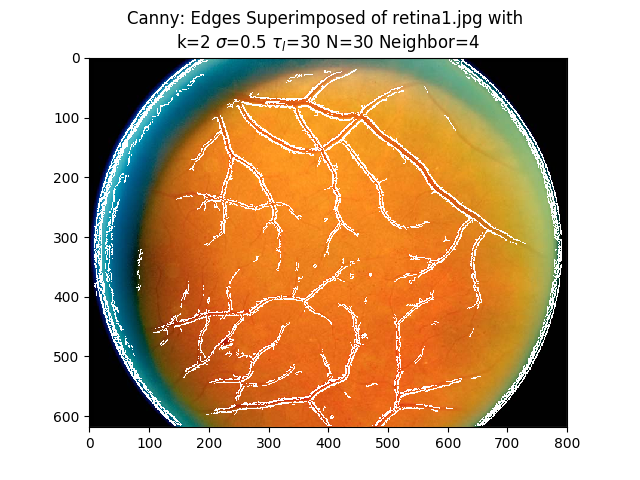
\includegraphics[width=.45\textwidth, height=.45\textheight]{canny_fig/retina1.jpg_fig5_0.png}\vspace{1pt}
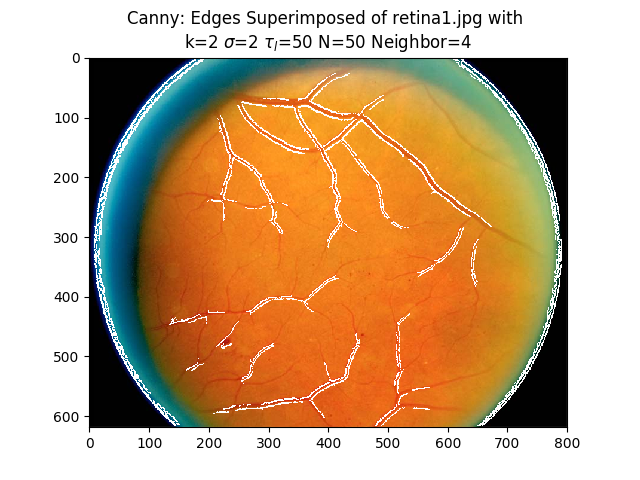
\includegraphics[width=.45\textwidth, height=.45\textheight]{canny_fig/retina1.jpg_fig5_4.png}\vfill
\end{column}
\end{columns}\vfill
\end{frame}

\begin{frame}
\frametitle{\textbf{Canny:} Result and Contrast}
\begin{columns}[T] % align columns
\begin{column}{\textwidth}
\centering
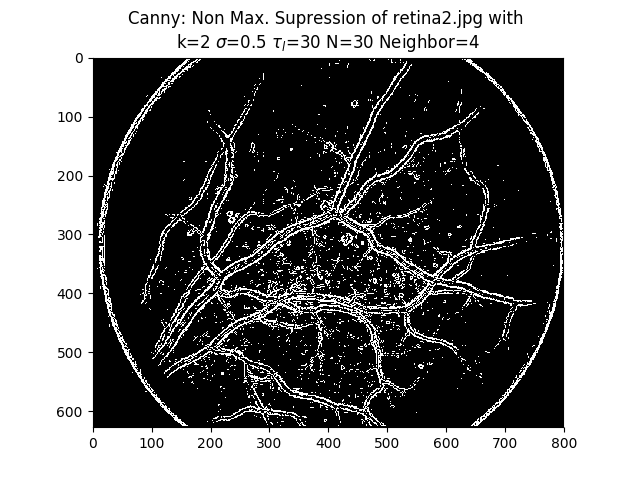
\includegraphics[width=.45\textwidth, height=.45\textheight]{canny_fig/retina2.jpg_fig2_1.png}\vspace{1pt}
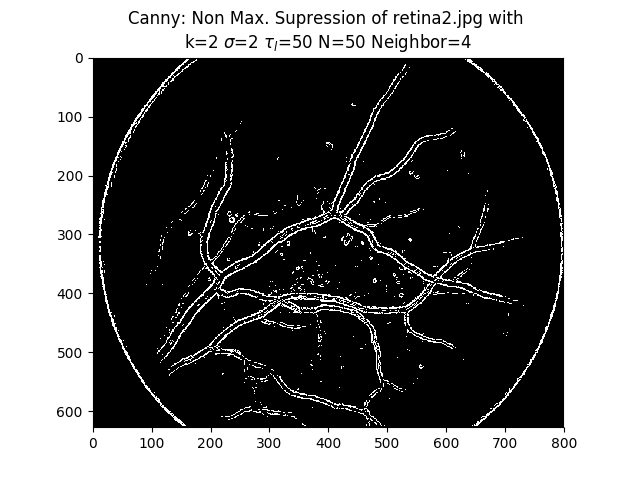
\includegraphics[width=.45\textwidth, height=.45\textheight]{canny_fig/retina2.jpg_fig2_5.png}\vfill
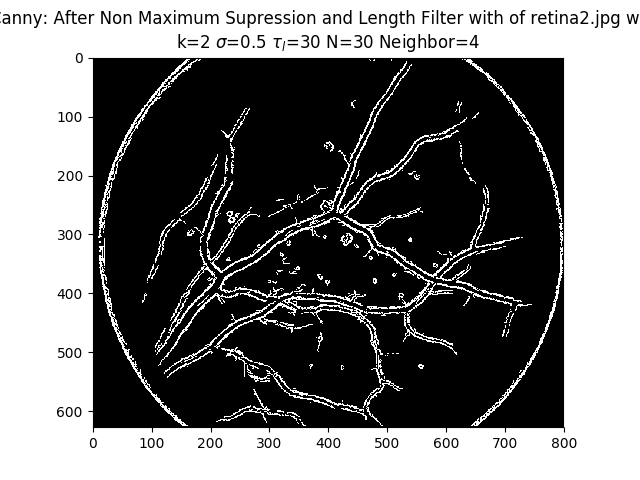
\includegraphics[width=.45\textwidth, height=.45\textheight]{canny_fig/retina2.jpg_fig3_1.png}\vspace{1pt}
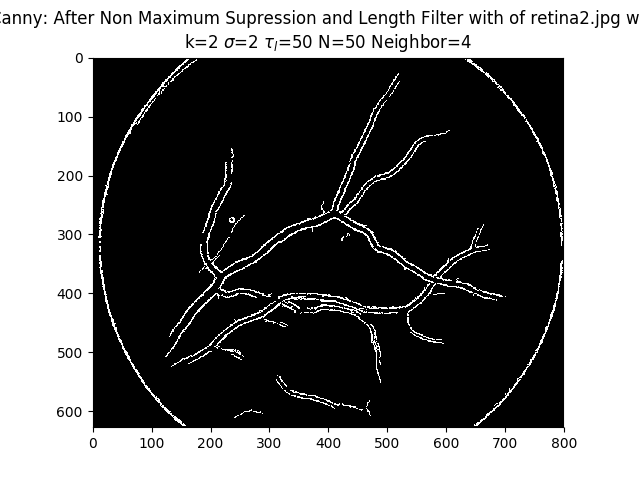
\includegraphics[width=.45\textwidth, height=.45\textheight]{canny_fig/retina2.jpg_fig3_5.png}\vfill
\end{column}
\end{columns}\vfill
\end{frame}

\begin{frame}
\frametitle{\textbf{Canny:} Result and Contrast}
\begin{columns}[T] % align columns
\begin{column}{\textwidth}
\centering
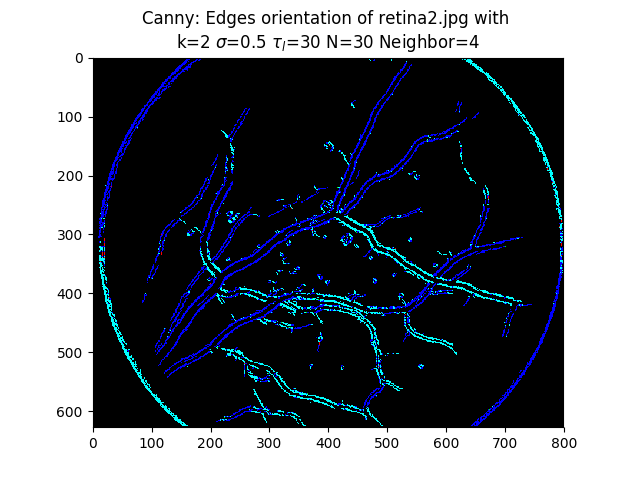
\includegraphics[width=.45\textwidth, height=.45\textheight]{canny_fig/retina2.jpg_fig4_1.png}\vspace{1pt}
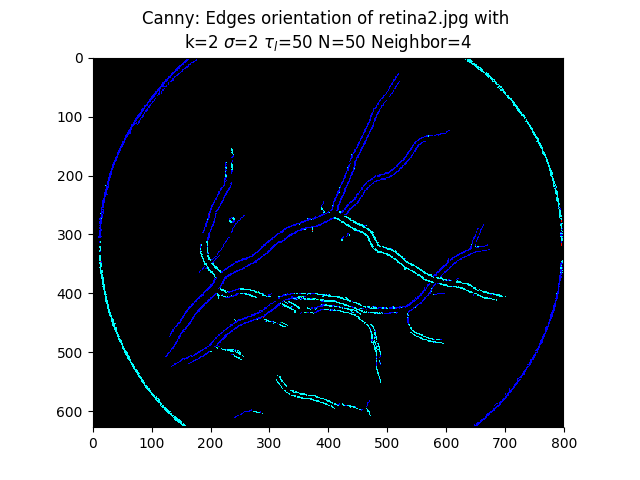
\includegraphics[width=.45\textwidth, height=.45\textheight]{canny_fig/retina2.jpg_fig4_5.png}\vfill
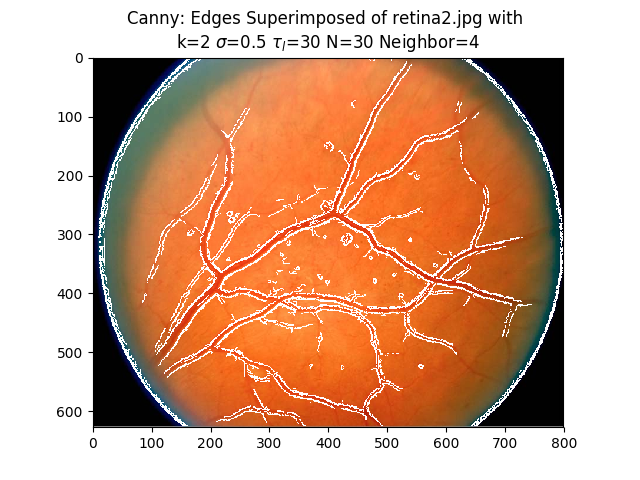
\includegraphics[width=.45\textwidth, height=.45\textheight]{canny_fig/retina2.jpg_fig5_1.png}\vspace{1pt}
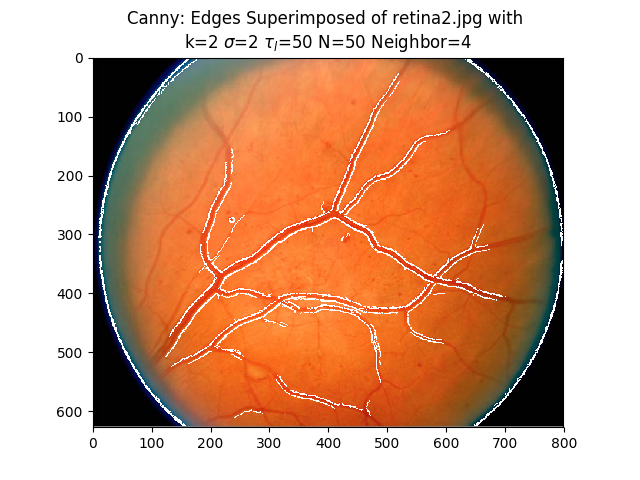
\includegraphics[width=.45\textwidth, height=.45\textheight]{canny_fig/retina2.jpg_fig5_5.png}\vfill
\end{column}
\end{columns}\vfill
\end{frame}



\begin{frame}
\frametitle{\textbf{Canny:} Result and Contrast}
\begin{columns}[T] % align columns
\begin{column}{\textwidth}
\centering
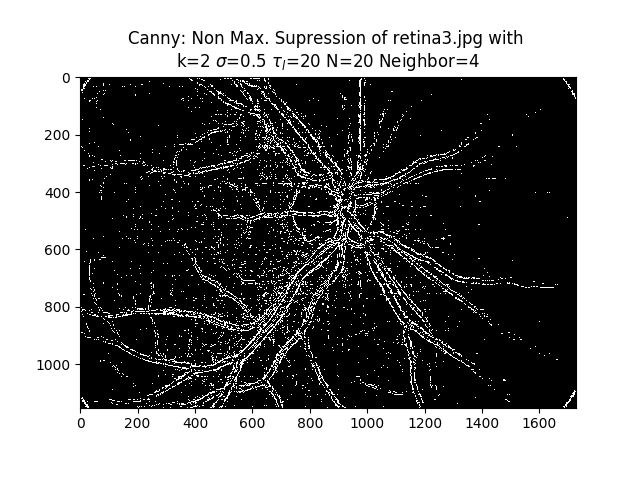
\includegraphics[width=.45\textwidth, height=.45\textheight]{canny_fig/retina3.jpg_fig2_2.png}\vspace{1pt}
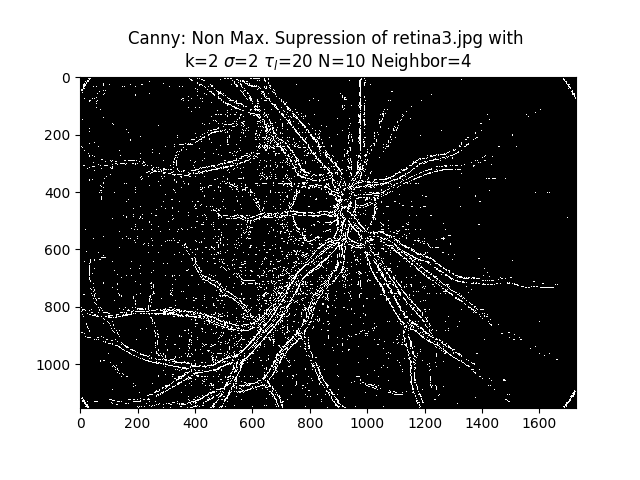
\includegraphics[width=.45\textwidth, height=.45\textheight]{canny_fig/retina3.jpg_fig2_6.png}\vfill
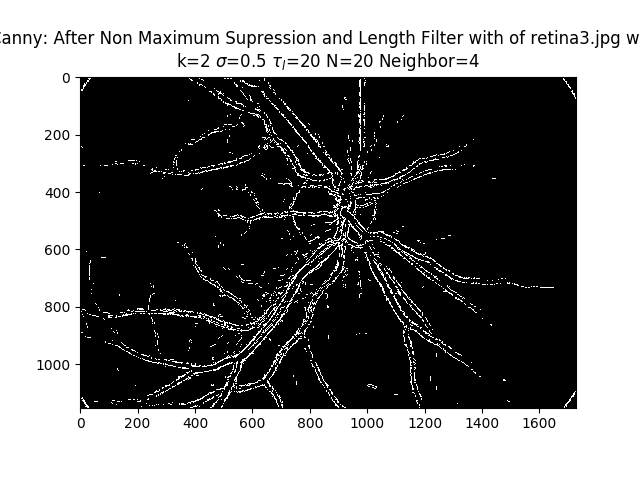
\includegraphics[width=.45\textwidth, height=.45\textheight]{canny_fig/retina3.jpg_fig3_2.png}\vspace{1pt}
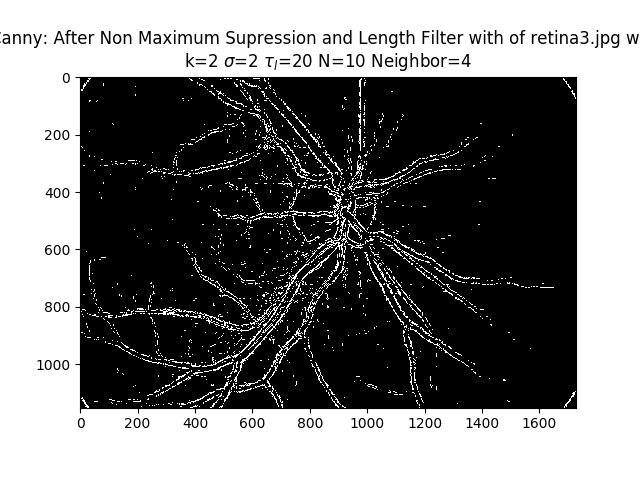
\includegraphics[width=.45\textwidth, height=.45\textheight]{canny_fig/retina3.jpg_fig3_6.png}\vfill
\end{column}
\end{columns}\vfill
\end{frame}

\begin{frame}
\frametitle{\textbf{Canny:} Result and Contrast}
\begin{columns}[T] % align columns
\begin{column}{\textwidth}
\centering
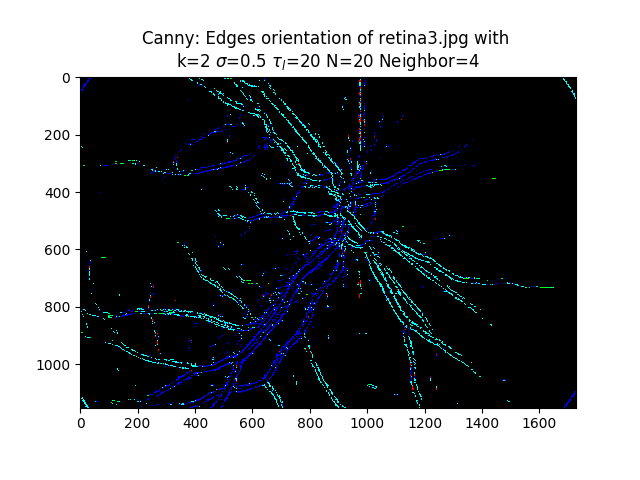
\includegraphics[width=.45\textwidth, height=.45\textheight]{canny_fig/retina3.jpg_fig4_2.png}\vspace{1pt}
\includegraphics[width=.45\textwidth, height=.45\textheight]{canny_fig/retina3.jpg_fig4_6.png}\vfill
\includegraphics[width=.45\textwidth, height=.45\textheight]{canny_fig/retina3.jpg_fig5_2.png}\vspace{1pt}
\includegraphics[width=.45\textwidth, height=.45\textheight]{canny_fig/retina3.jpg_fig5_6.png}\vfill
\end{column}
\end{columns}\vfill
\end{frame}

\begin{frame}
\frametitle{\textbf{Canny:} Result and Contrast}
\begin{columns}[T] % align columns
\begin{column}{\textwidth}
\centering
\includegraphics[width=.45\textwidth, height=.45\textheight]{canny_fig/retina4.jpg_fig2_3.png}\vspace{1pt}
\includegraphics[width=.45\textwidth, height=.45\textheight]{canny_fig/retina4.jpg_fig2_7.png}\vfill
\includegraphics[width=.45\textwidth, height=.45\textheight]{canny_fig/retina4.jpg_fig3_3.png}\vspace{1pt}
\includegraphics[width=.45\textwidth, height=.45\textheight]{canny_fig/retina4.jpg_fig3_7.png}\vfill
\end{column}
\end{columns}\vfill
\end{frame}

\begin{frame}
\frametitle{\textbf{Canny:} Result and Contrast}
\begin{columns}[T] % align columns
\begin{column}{\textwidth}
\centering
\includegraphics[width=.45\textwidth, height=.45\textheight]{canny_fig/retina4.jpg_fig4_3.png}\vspace{1pt}
\includegraphics[width=.45\textwidth, height=.45\textheight]{canny_fig/retina4.jpg_fig4_7.png}\vfill
\includegraphics[width=.45\textwidth, height=.45\textheight]{canny_fig/retina4.jpg_fig5_3.png}\vspace{1pt}
\includegraphics[width=.45\textwidth, height=.45\textheight]{canny_fig/retina4.jpg_fig5_7.png}\vfill
\end{column}
\end{columns}\vfill
\end{frame}

\subsection{Matched Filter}
\begin{frame}
\frametitle{\textbf{Match:} Result and Contrast}
\begin{columns}[T] % align columns
\begin{column}{\textwidth}
\centering
\includegraphics[width=.45\textwidth, height=.45\textheight]{match_fig/retina1.jpg_fig1_0.png}\vspace{1pt}
\includegraphics[width=.45\textwidth, height=.45\textheight]{match_fig/retina1.jpg_fig1_4.png}\vfill
\includegraphics[width=.45\textwidth, height=.45\textheight]{match_fig/retina1.jpg_fig3_0.png}\vspace{1pt}
\includegraphics[width=.45\textwidth, height=.45\textheight]{match_fig/retina1.jpg_fig3_4.png}\vfill
\end{column}
\end{columns}\vfill
\end{frame}

\begin{frame}
\frametitle{\textbf{Match:} Result and Contrast}
\begin{columns}[T] % align columns
\begin{column}{\textwidth}
\centering
\includegraphics[width=.45\textwidth, height=.45\textheight]{match_fig/retina1.jpg_fig4_0.png}\vspace{1pt}
\includegraphics[width=.45\textwidth, height=.45\textheight]{match_fig/retina1.jpg_fig4_4.png}\vfill
\includegraphics[width=.45\textwidth, height=.45\textheight]{match_fig/retina1.jpg_fig5_0.png}\vspace{1pt}
\includegraphics[width=.45\textwidth, height=.45\textheight]{match_fig/retina1.jpg_fig5_4.png}\vfill
\end{column}
\end{columns}\vfill
\end{frame}

\begin{frame}
\frametitle{\textbf{Match:} Result and Contrast}
\begin{columns}[T] % align columns
\begin{column}{\textwidth}
\centering
\includegraphics[width=.45\textwidth, height=.45\textheight]{match_fig/retina1.jpg_fig6_0.png}\vspace{1pt}
\includegraphics[width=.45\textwidth, height=.45\textheight]{match_fig/retina1.jpg_fig6_4.png}\vfill
\includegraphics[width=.45\textwidth, height=.45\textheight]{match_fig/retina1.jpg_fig7_0.png}\vspace{1pt}
\includegraphics[width=.45\textwidth, height=.45\textheight]{match_fig/retina1.jpg_fig7_4.png}\vfill
\end{column}
\end{columns}\vfill
\end{frame}

\begin{frame}
\frametitle{\textbf{Match:} Result and Contrast}
\begin{columns}[T] % align columns
\begin{column}{\textwidth}
\centering
\includegraphics[width=.45\textwidth, height=.45\textheight]{match_fig/retina1.jpg_fig8_0.png}\vspace{1pt}
\includegraphics[width=.45\textwidth, height=.45\textheight]{match_fig/retina1.jpg_fig8_4.png}\vfill
\includegraphics[width=.45\textwidth, height=.45\textheight]{match_fig/retina1.jpg_fig9_0.png}\vspace{1pt}
\includegraphics[width=.45\textwidth, height=.45\textheight]{match_fig/retina1.jpg_fig9_4.png}\vfill
\end{column}
\end{columns}\vfill
\end{frame}

\begin{frame}
\frametitle{\textbf{Match:} Result and Contrast}
\begin{columns}[T] % align columns
\begin{column}{\textwidth}
\centering
\includegraphics[width=.45\textwidth, height=.45\textheight]{match_fig/retina1.jpg_fig6_0.png}\vspace{1pt}
\includegraphics[width=.45\textwidth, height=.45\textheight]{match_fig/retina1.jpg_fig6_4.png}\vfill
\includegraphics[width=.45\textwidth, height=.45\textheight]{match_fig/retina1.jpg_fig7_0.png}\vspace{1pt}
\includegraphics[width=.45\textwidth, height=.45\textheight]{match_fig/retina1.jpg_fig7_4.png}\vfill
\end{column}
\end{columns}\vfill
\end{frame}

\begin{frame}
\frametitle{\textbf{Match:} Result and Contrast}
\begin{columns}[T] % align columns
\begin{column}{\textwidth}
\centering
\includegraphics[width=.45\textwidth, height=.45\textheight]{match_fig/retina2.jpg_fig5_1.png}\vspace{1pt}
\includegraphics[width=.45\textwidth, height=.45\textheight]{match_fig/retina2.jpg_fig5_5.png}\vfill
\includegraphics[width=.45\textwidth, height=.45\textheight]{match_fig/retina2.jpg_fig6_1.png}\vspace{1pt}
\includegraphics[width=.45\textwidth, height=.45\textheight]{match_fig/retina2.jpg_fig6_5.png}\vfill
\end{column}
\end{columns}\vfill
\end{frame}

\begin{frame}
\frametitle{\textbf{Match:} Result and Contrast}
\begin{columns}[T] % align columns
\begin{column}{\textwidth}
\centering
\includegraphics[width=.45\textwidth, height=.45\textheight]{match_fig/retina2.jpg_fig8_1.png}\vspace{1pt}
\includegraphics[width=.45\textwidth, height=.45\textheight]{match_fig/retina2.jpg_fig8_5.png}\vfill
\includegraphics[width=.45\textwidth, height=.45\textheight]{match_fig/retina2.jpg_fig9_1.png}\vspace{1pt}
\includegraphics[width=.45\textwidth, height=.45\textheight]{match_fig/retina2.jpg_fig9_5.png}\vfill
\end{column}
\end{columns}\vfill
\end{frame}

\begin{frame}
\frametitle{\textbf{Match:} Result and Contrast}
\begin{columns}[T] % align columns
\begin{column}{\textwidth}
\centering
\includegraphics[width=.45\textwidth, height=.45\textheight]{match_fig/retina3.jpg_fig5_2.png}\vspace{1pt}
\includegraphics[width=.45\textwidth, height=.45\textheight]{match_fig/retina3.jpg_fig5_6.png}\vfill
\includegraphics[width=.45\textwidth, height=.45\textheight]{match_fig/retina3.jpg_fig6_2.png}\vspace{1pt}
\includegraphics[width=.45\textwidth, height=.45\textheight]{match_fig/retina3.jpg_fig6_6.png}\vfill
\end{column}
\end{columns}\vfill
\end{frame}

\begin{frame}
\frametitle{\textbf{Match:} Result and Contrast}
\begin{columns}[T] % align columns
\begin{column}{\textwidth}
\centering
\includegraphics[width=.45\textwidth, height=.45\textheight]{match_fig/retina3.jpg_fig8_2.png}\vspace{1pt}
\includegraphics[width=.45\textwidth, height=.45\textheight]{match_fig/retina3.jpg_fig8_6.png}\vfill
\includegraphics[width=.45\textwidth, height=.45\textheight]{match_fig/retina3.jpg_fig9_2.png}\vspace{1pt}
\includegraphics[width=.45\textwidth, height=.45\textheight]{match_fig/retina3.jpg_fig9_6.png}\vfill
\end{column}
\end{columns}\vfill
\end{frame}

\begin{frame}
\frametitle{\textbf{Match:} Result and Contrast}
\begin{columns}[T] % align columns
\begin{column}{\textwidth}
\centering
\includegraphics[width=.45\textwidth, height=.45\textheight]{match_fig/retina4.jpg_fig5_3.png}\vspace{1pt}
\includegraphics[width=.45\textwidth, height=.45\textheight]{match_fig/retina4.jpg_fig5_7.png}\vfill
\includegraphics[width=.45\textwidth, height=.45\textheight]{match_fig/retina4.jpg_fig6_3.png}\vspace{1pt}
\includegraphics[width=.45\textwidth, height=.45\textheight]{match_fig/retina4.jpg_fig6_7.png}\vfill
\end{column}
\end{columns}\vfill
\end{frame}

\begin{frame}
\frametitle{\textbf{Match:} Result and Contrast}
\begin{columns}[T] % align columns
\begin{column}{\textwidth}
\centering
\includegraphics[width=.45\textwidth, height=.45\textheight]{match_fig/retina4.jpg_fig8_3.png}\vspace{1pt}
\includegraphics[width=.45\textwidth, height=.45\textheight]{match_fig/retina4.jpg_fig8_7.png}\vfill
\includegraphics[width=.45\textwidth, height=.45\textheight]{match_fig/retina4.jpg_fig9_3.png}\vspace{1pt}
\includegraphics[width=.45\textwidth, height=.45\textheight]{match_fig/retina4.jpg_fig9_7.png}\vfill
\end{column}
\end{columns}\vfill
\end{frame}


\begin{frame}
\frametitle{Final Comparison}
\begin{columns}[T] % align columns
\begin{column}{\textwidth}
\centering
\includegraphics[width=.28\textwidth, height=.24\textheight]{log_fig/retina1.jpg_fig6_4.png}
\includegraphics[width=.28\textwidth, height=.24\textheight]{canny_fig/retina1.jpg_fig5_0.png}
\includegraphics[width=.28\textwidth, height=.24\textheight]{match_fig/retina1.jpg_fig9_0.png}\vfill
\includegraphics[width=.28\textwidth, height=.24\textheight]{log_fig/retina2.jpg_fig6_5.png}
\includegraphics[width=.28\textwidth, height=.24\textheight]{canny_fig/retina2.jpg_fig5_1.png}
\includegraphics[width=.28\textwidth, height=.24\textheight]{match_fig/retina2.jpg_fig9_1.png}\vfill
\includegraphics[width=.28\textwidth, height=.24\textheight]{log_fig/retina3.jpg_fig6_3.png}
\includegraphics[width=.28\textwidth, height=.24\textheight]{canny_fig/retina3.jpg_fig5_2.png}
\includegraphics[width=.28\textwidth, height=.24\textheight]{match_fig/retina3.jpg_fig9_6.png}\vfill
\includegraphics[width=.28\textwidth, height=.24\textheight]{log_fig/retina4.jpg_fig6_8.png}
\includegraphics[width=.28\textwidth, height=.24\textheight]{canny_fig/retina4.jpg_fig5_3.png}
\includegraphics[width=.28\textwidth, height=.24\textheight]{match_fig/retina4.jpg_fig9_7.png}\vfill
\end{column}
\end{columns}\vfill
\end{frame}

\section{Conclusion}
\begin{frame}
\frametitle{Conclusion}
\begin{itemize}
	\item In this project, we have studied the Edge detection using LoG, Canny and Match filter Method
	\item LoG is simplistic in design and can but can not capture blood vessel rather captures the edges it is also spatial only does not give orientation information
	\item Canny gives spatial and orientation information. Besides there are some important criteria like signal to noise ratio, low false positive rate makes it attractive. However non Maximal Suppression can be time consuming.
	\item Matched filter gives more insight about the edge and better in detecting blood vessel. However manual design of filters may require efforts.
\end{itemize}
\end{frame}

\begin{frame}
\frametitle{Additional Work}
\begin{itemize}
	\item Developed my python implementation of Matlab BWLABEL
	\item My implementation can be found at LoG implementation py\_bwlabel
	\item py\_bwlabel is notoriously slow
	\item I figured out Matlab and skimage.measure.label uses bitwise optimization
	\item I had to use unofficial python package bwmorph\_thin of BWMORPH as well
\end{itemize}
\end{frame}

% ------------------------------------------------------------------------------------------------------------------

% ------------------------------------------------------------------------------------------------------------------

\end{document}

